\chapter{Teknisk Design}
\label{chap:technical}


\section{Teknologi}
Hele prosjektet har blitt skrevet i Python, vi valgte å utvikle programvaren i Eclipse PyDev utvidelsen. TKinter ble brukt til utvikling av GUI, vi valgte Tkinter fordi det var oversiktlig og lett å ta i bruk. Vi bruker MatPlotLib til å presentere grafen i 2D versjonen. Vi valgte å bruke denne fordi den var kompatibel med Tkinter. Vi valgte å skrive koden i Python fordi det er et høynivåspråk som er utrolig effektivt. Det kan spesielt håndtere grafiske 2D og 3D visninger. \\ \\

\section{System Arkitektur}
Vi har valgt å ta i bruk MVC som står for Model View Controller. MVC er en arkitektur modell som deler programvaren opp i tre forskjellige grupper. Disse gruppene representere en del av programvaren og skal gi en flyt av informasjon. Modellen består av Model som håndterer informasjon og logistikk.  View er all visning av informasjon, dette kan være ting som bilder, video, tekst eller diagram. Controller håndtere all informasjon som brukeren gir til programvaren, som blir gjort om til kommandoer som Model kan bruke.[2]

\begin{figure}[h]
    \centering
    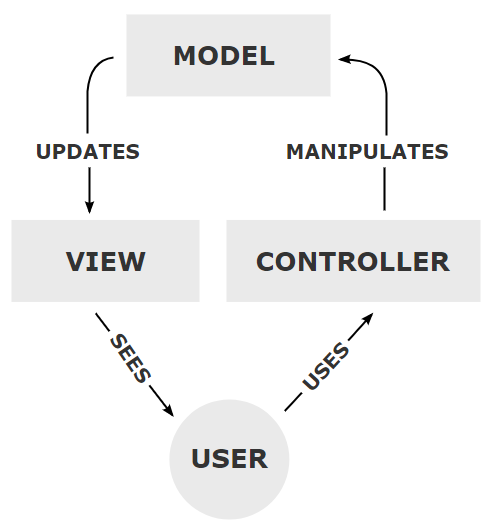
\includegraphics[width=8cm, height=8cm,]{MVC}
    \caption{Model View Controller diagram}
    \label{fig:my_label}
\end{figure}




\section{Arkitektur oversikt}
\subsection{Vår implementasjon av MVC}
I denne delen vil vi gi en oversikt over arkitekturmodellen vi har valgt å bruke. Nammo satte ikke noen krav til arkitekturen, de kom kun med en liste funksjonaliteter de ønsket oppfylt. Dette ga oss en stor frihet over hvordan vi kunne strukturere koden vår. Vi valgte å strukturere koden vår etter en MVC modell som har blitt kort forklart over. Vi valgte å bruke denne på grunn av dens vidsprede bruk i industrien, vår tidligere erfaring med arkitektur modellen og fordi oppgaven vår kunne naturlig deles etter MVC prinsippene. \\ \\
Arkitektur Modellen skal gjøre kildekoden oversiktlighet, som vil gjøre det lettere for nye utviklere å jobbe videre på programvaren etter dette prosjektet. Dette er vesentlig for programvaren fordi den er kun en tidlig utgave av det Nammo ønsker. Da det tidlig ble klart at vi ikke ville kunne implementere alle funksjonalitetene Nammo ønsket har vi hatt et stort fokus på å skape oversiktlig og velstrukturert kode. \\ \\
I Model delen har vi lagt inn dataobjektene, linjestykker og forhåndsdefinerte former som stjerner og tankveggen. De forhåndsdefinerte formene er satt sammen av linjestykker gitt vise parameter, og inneholder også data relatert logikk. Data relatert logikk sjekker at de gitte parameterene er innenfor gitte grenser, som at en stjernearm ikke er lengre enn radiusen til tankveggen.\\ \\
I View delen vil modellen og dataene etter simuleringen vises, og brukeren kan endre parameterene for modellen. Denne delen inneholder ikke noe logikk, da den kun mottar og viser data fra Controller delen og mottar og videresender data fra brukeren.\\ \\
I Controller delen skjer all applikasjonslogikken, som flytting av linjestykker etter som brennstoffet brenner opp og utregning av overflate og areal. Denne delen vil også mota brukerdata fra View delen og skape dataobjekter fra Model delen basert på disse dataene. De mest resursintensive delene av programmet skjer i denne delen da flyttingen av linjestykkene kan gi mange feil og derfor blir det her kjørt mange sjekker for å fjerne disse potensielle feilene.

\subsection{Klasse oversikt}
Klassen mover inneholder data om hvor langt hvert steg skal flytte linjestykkene, og hvor mange steg den har flyttet. Klassens viktigste funksjon er moveStep som flytter hvert linjestykke og kaller alle hjelpe funksjonene som sørger for at den nye formen etter flyttingen er riktig.\\ \\
Klassen lineSegment definerer et linjestykke med to endepunkt, og den beregner også lengden til linjestykket og den normaliserte normalen. Klassen innholder en del funksjoner for interaksjon med andre linjestykker, som å sjekke om to linjestykker er like, eller om de krysser hverandre.\\ \\
Klasser i shapes filen beskriver diverse former som blir brukt til skape stjerneformene og tankveggen i modelleringen. Vi her bare beskrive klasssen paraStar, da alle disse klassene er konseptuelt like og bare er ulike i hvilke former de skaper.\\ \\
Klassen paraStar skaper et dataobjekt med alle parameterene for å skape en halv stjernearm fra en stjerne med parallelle stjernearmer. Den inneholder funksjoner for å sette disse parameterene og en funksjon som generer den halve stjernearmen og returnerer en matrise med linjestykkene som beskriver figuren.\\ \\

\section{Språk og Rammeverk}

\subsection{Python}
Python er et høynivå språk utviklet på starten av 90 tallet. Python ble laget med filosofien som legger vekt på leselighet. Hovedsakelig ved bruk av mellomrom til å definere kode blokker i motsetning til semikolon og krøllparentes som blir brukt i mer tradisjonelle språk. Språket gir brukeren muligheten til å uttrykke begreper over få linjer kode i forhold til mer tradisjonelle språk som C++ eller Java. Pythons kompakte og effektive kode gjør det til et godt verktøy for utvikling av prototyper. Vi valgte å skrive programvaren vår i Python på grunn av språkets høynivå og mulighet til å presentere 3D modeller. Når vi undersøkt hvilket hvilket språk vi skulle ta i bruk ble Python anbefalt av veileder. Det var en positiv opplevelse å gå over til et høynivå språk, selv om mangel av semikolon og krøllparentes var uvant og bruke av mellomrom var litt av en overgang var vi fornøyde med valget. 

\subsection{Eclipce Pydev}
Når vi hadde funnet språket vi skulle utvikle programvaren i måtte vi velge et IDE. Vi valgte å bruke Eclipse med tredje part plug in Pydev. Eclipse er originalt brukt til utvikling av Java, men med dens enorm støtte fra tredjepart utviklere som tilbyr plug in, valgte vi å bruke Eclipse. Pydev er en av de mest brukte IDE for Python, Noe som ga oss en trygghet når vi møtte på problemer ettersom det var allerede noen som hadde møtt på det samme problemet før oss, og hadde funnet en løsning på problemet.


\subsection{MatPlotLib}
matPlotLib er et bibliotek utviklet for Python og den matematiske utvidelse NumPy. Den gir en objektorientert API som gir oss muligheten til å presentere en graf gjennom bruken av et GUI verktøy som Tkinter, qt, GTK+. MatPlotLib var lett å bruke sammen med Tkinter, vi bruke funksjonen pack() som satt opp grafen i Tkinter. Dette gjorde at vi raskt fikk opp funksjonaliteten, men design ble vanskelig. Ettersom vi brukte funksjonen pack() hadde vi lite kontroll over hvor den havnet. Vi prøvde å bruke en “grid” løsning, dette skapte kun problemer, og vi fikk ikke lengre vist grafen som vi ønsket.


\subsection{Tkinter}
Vi måtte ha en måte å presentere grafen vå på en brukervennlig måte som trakk brukeren til å bruke programvaren. Vi valgte å bruke Tkinter fordi den var kompatibel med MatPlotLib, i tillegg til at det var en lav læringskurve.